%%% Fiktivní kapitola s ukázkami sazby

\chapter{Analýza problému a jeho řešení}

V této kapitole je detailně popsán problém a způsoby jeho navrženého a současného řešení.

\section{Popis problému odhadu zpoždění}

Spoje které zajištˇují hromadnou dopravu se řídí jízdními řády, které určují jejich trasu a udávají časy příjezdu a odjezdu do daných zastávek. Toto jsou zpravidla jediné refenční body u kterých je možno zjistit skutečné zpoždění, nebo předjetí (dále uvažováno jako zpoždění se zápornou hodnotou).

\bigbreak

Vzhledem k tom, že délka trasy mezi dvěma refernčními body nezříka dosahuje i několika desítek kilometrů (TODO spocitat prumer a median), kde sice mohou vznikat mimořáné události, ale ve většině případů je ovlivněna pouze obvyklým provozem v dané denní době, je potřeba navrhnout systém na odhat zpoždění v půběhu jízdy mezi těmito body.

\bigbreak

Tento odhad je nutné počítat v reálném čase, tak aby uživatelé byli dobře informování o stavu jejich spoje. A proto je potřeba zpracovávat data okamžitě po jejich vydání, spočítat odhad zpoždění a vystavit tyto data veřejně. Vzhledem k tomu, že tyto data velmi rychle zastarávají je nutné provádět tento proces co možná nejrychleji.

\bigbreak

Pro vyjasnění je potřeba uvést, že se systém nesnaží předpovědět zpoždění, které spoj může nabrat vzhledem k dosavadnímu průběhy trasy. Ale snaží se odhadnou zpoždění v danném bodě na trase vzhledem k obvyklému profilu jízdy.

TODO obrazek nelinearni trasy

\subsection{Současná řešení}

Takový algoritmus na odhat aktuálního zpoždění mezi dvěma referenčními body již exituje a je zakomponován v systému, ze kterého se čerpají data pro tuto práci. (Detailní popis dat uveden v kapitole ~\ref{chapter:TODO later}.) Nicméně nezohledňuje základní parametry průběhu trasy. Tento algoritmus nahlíží na postup vozidla na trase jako na lineární funkci vůči času. Je ovšem zřejmé, že rychlost vozidel není konstantní, neboli doba jízdy není linárně závislá na ujeté vzdálenosti.

\section{Analýza požadavků na uživatelskou aplikaci}

Součástí práce je i vizualizace spočítaných dat. Jinými slovy nástroj umožňující přístup uživatelů ke spočítaným datům.

\subsubsection{Funkční požadavky}

\begin{itemize}
	\item Aplikace vykreslí interaktivní mapu Prahy a širšího okolí, kterou bude možné posouvat či zoomovat. V této mapě budou zobrazeny jednotlivé vozidla na aktuálních pozicích a budou se automaticky posouvat po mapě, tak jak se pohybují ve skutečnosti.

	\item Po kliknutí na vozidlo se zobrazí jeho celá trasa včetně zastávek a jeho dopočítaného zpoždění.

	\item Po kliknutí na zastávku se zobrazí seznam spojů, které budou projíždět vybranou zastávkou a jejich trasy se vykreslí do mapy.

	\item Celá aplikace bude postavena na principu server -- client. Tedy serverová strana se postará o přístup k otevřeným datům o vozidlech a jejich uložení a také obsluhu požadavků klienta. Klientská část bude webová stránka poskytující služby popsané výše. Měla by být schopná zobrazit řádově tisíce vozidel.
\end{itemize}

\subsubsection{Nefunkční požadavky}

\begin{itemize}
	\item Serverová část bude napsaná v jazyce Python 3.

	\item Webová část bude napsaná pomocí jazyků pro webové technologie, převážně v JavaScriptu.

	\item Pro vykleslení mapy bude využita služba Mapbox.

	\item Ukládání dat na serverové straně bude řešeno MySQL databází.

	\item Pro algoritmus odhadu zpoždění na zákldě historických dat budou využity různé knihovny pro jazyk Python 3. Zejména pak scikit-learn a alphashape.

\end{itemize}

\subsubsection{Proces běhu aplikace}

Jak je již zmíněno aplikace bude využívat historická data, tedy bude nutné nechat aplikaci tato data nějakou dobu sbírat. Pro efektivní odhady by bylo vhodné mít uložené historické polohy vozidel alespoň z uplynulých několika týdnů.

\bigbreak

Avšak již v průběhu sběru dat může aplikace poskytovat základní službu a to vizualizování vozidel v mapě.

\subsection{Poskytovatelé mapových podkladů}

K takovému účelu nejlépe poslouží vykreslení aktuálních poloh vozidel do mapy, kde se po vyžádání uživatelem tyto data zobrazí.

\bigbreak

Za účelem vytvoření dostatečně přívětivé uživatelské aplikace je nezbytné využít některého z poskytovatelů mapových podkladů a zanést do něj získané informace.

\bigbreak

Jedním z těchto poskytovatelů je společnost Google, která má propracované mapové podklady a prostřednictvím služby Google Maps poskytuje pro tuto práci požadovanou službu. Další platformou je Mapbox, který poskytuje velmi podobné služby jako Google Maps. Nicméně narozdíl od Googlu využívá jako mapový podklad \gls{osm} {otevřená geografické data}. Protože smyslem práce je v co největší míře využít otevřená data je žádoucí využít právě Mapbox.

\bigbreak

TODO dokumentace mapbox, zeptat se jestli je to vubec nutne rozebirat

\subsection{Současná řešení}

Vizualizaci vozidel \gls{vhd} do mapy již nabízí několik portálů. Všechny jsou však poměrně strohé.

\subsubsection{Golemio}

Takovou mapu zobrazuje i samotný provozavatel datové platformy. Nicméně nejsou zde vidět ani čísla linek zobrazených autobusů, natož pak nějaké další informace.

\begin{figure}
  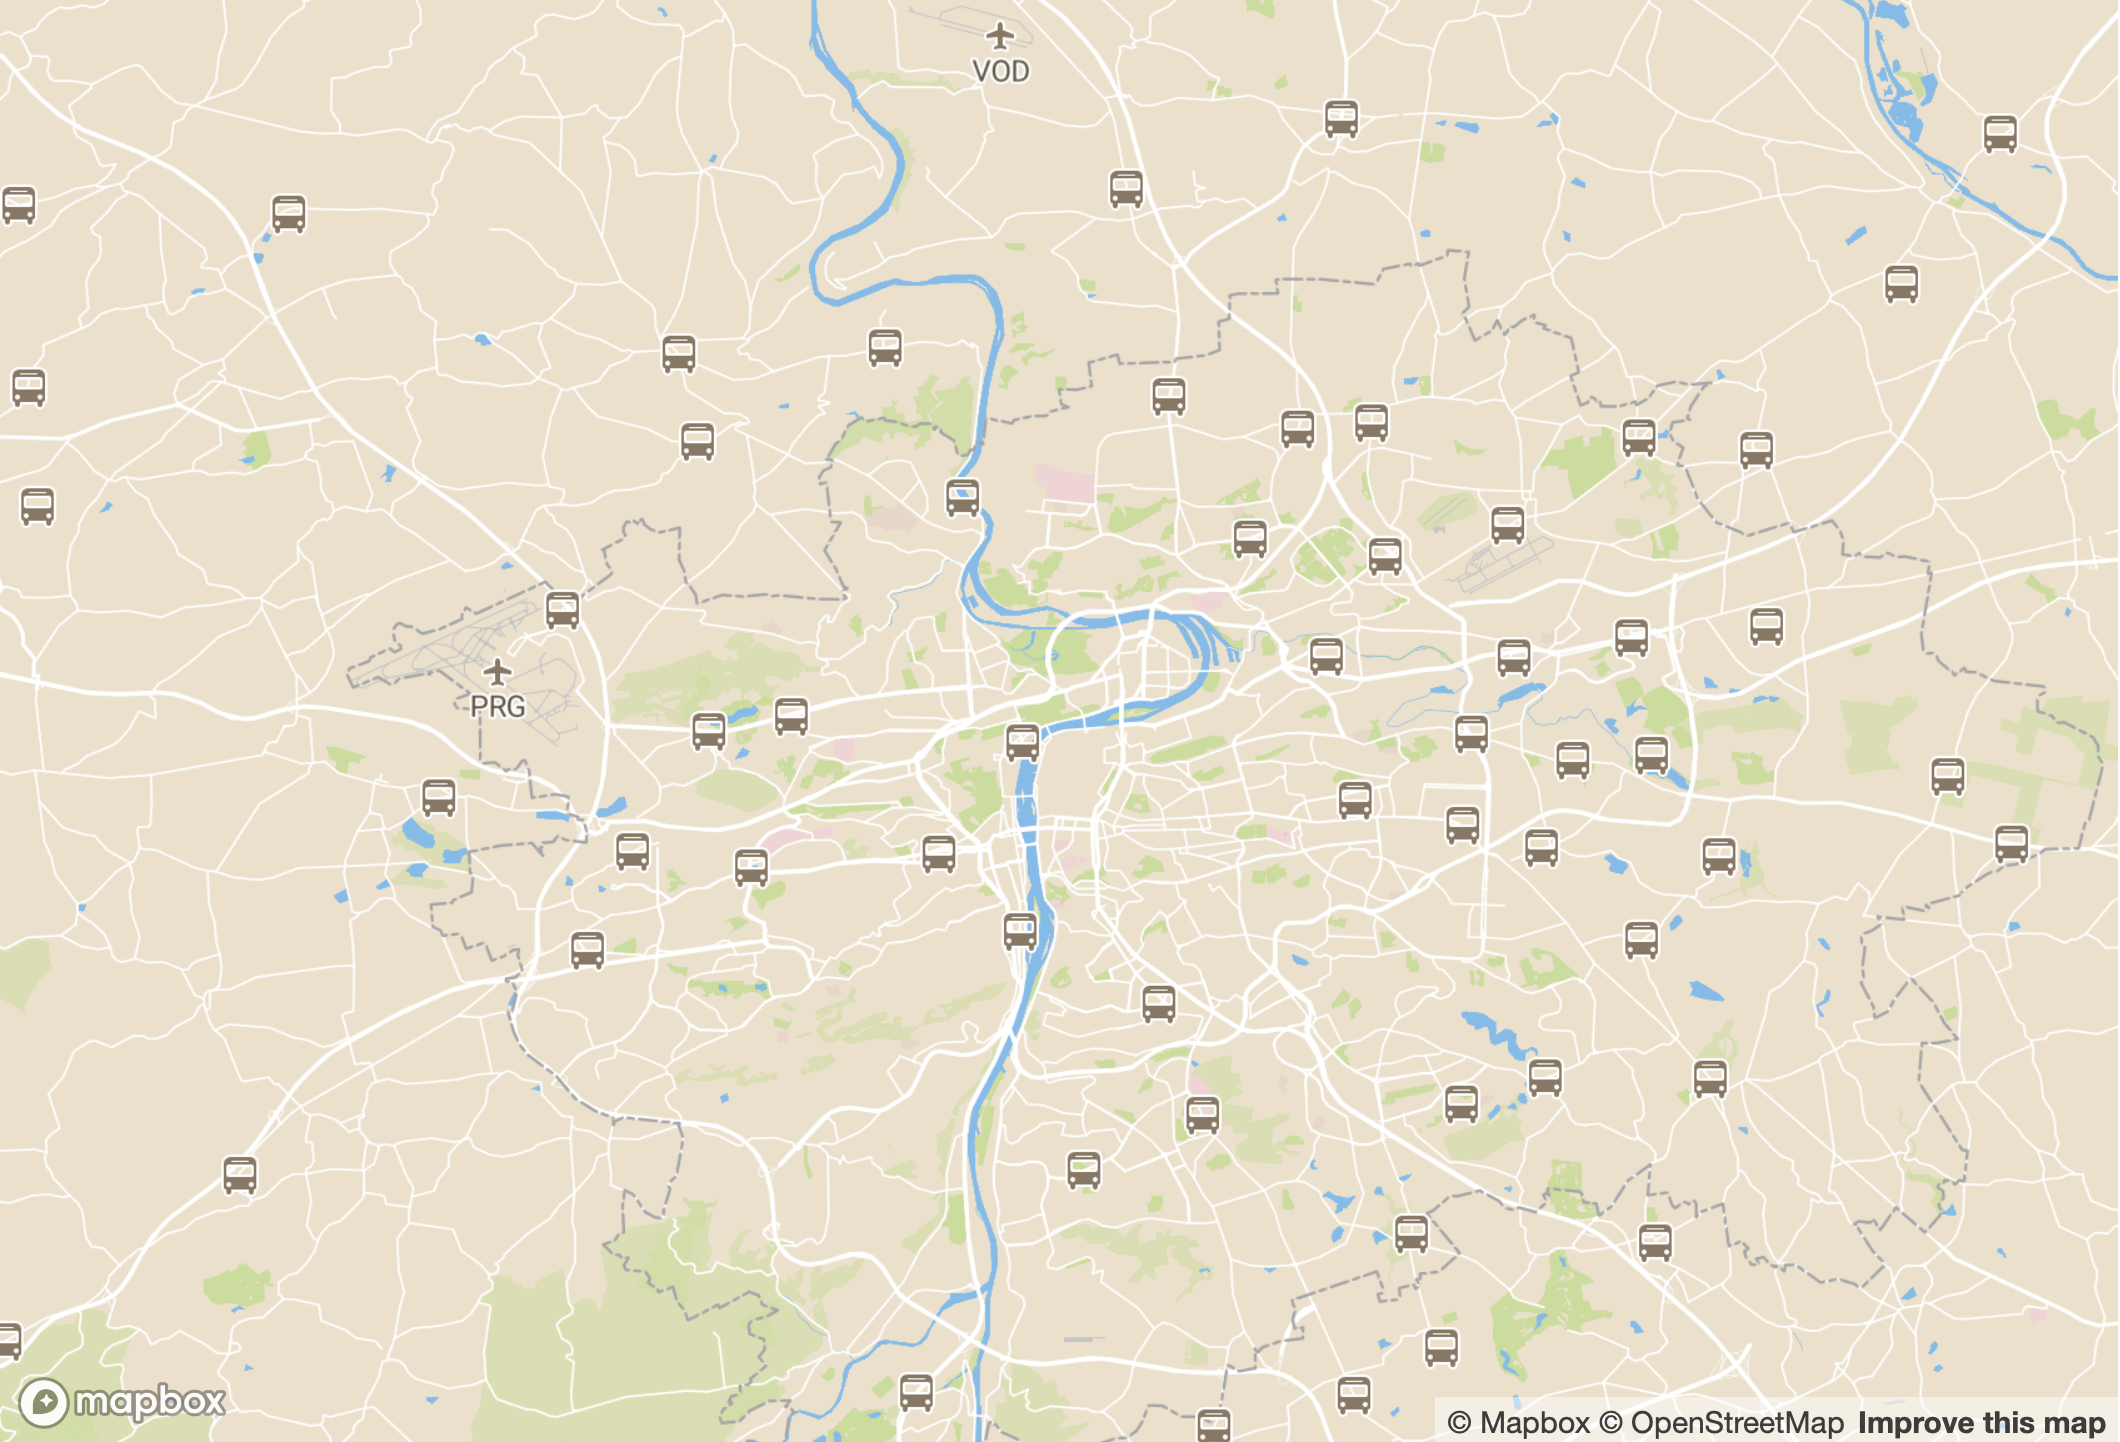
\includegraphics[width=\linewidth]{../img/golemio_mapa.png}
  \caption{Mapa z golemio.cz.}
  \label{fig:golemio_result}
\end{figure}

\subsubsection{Tram-bus}

Dalším poskytovatelem je portál tram-bus, který si vede o něco lépe. Ukazuje směr jízdy vozidel, čísla linek a po kliknutí informace o zpoždění a nejbližší zastávky. Pozn.: na mapě již jsou vidět spoje \gls{dpp}, protože v době psaní této práce již byly data veřejné.

\begin{figure}
  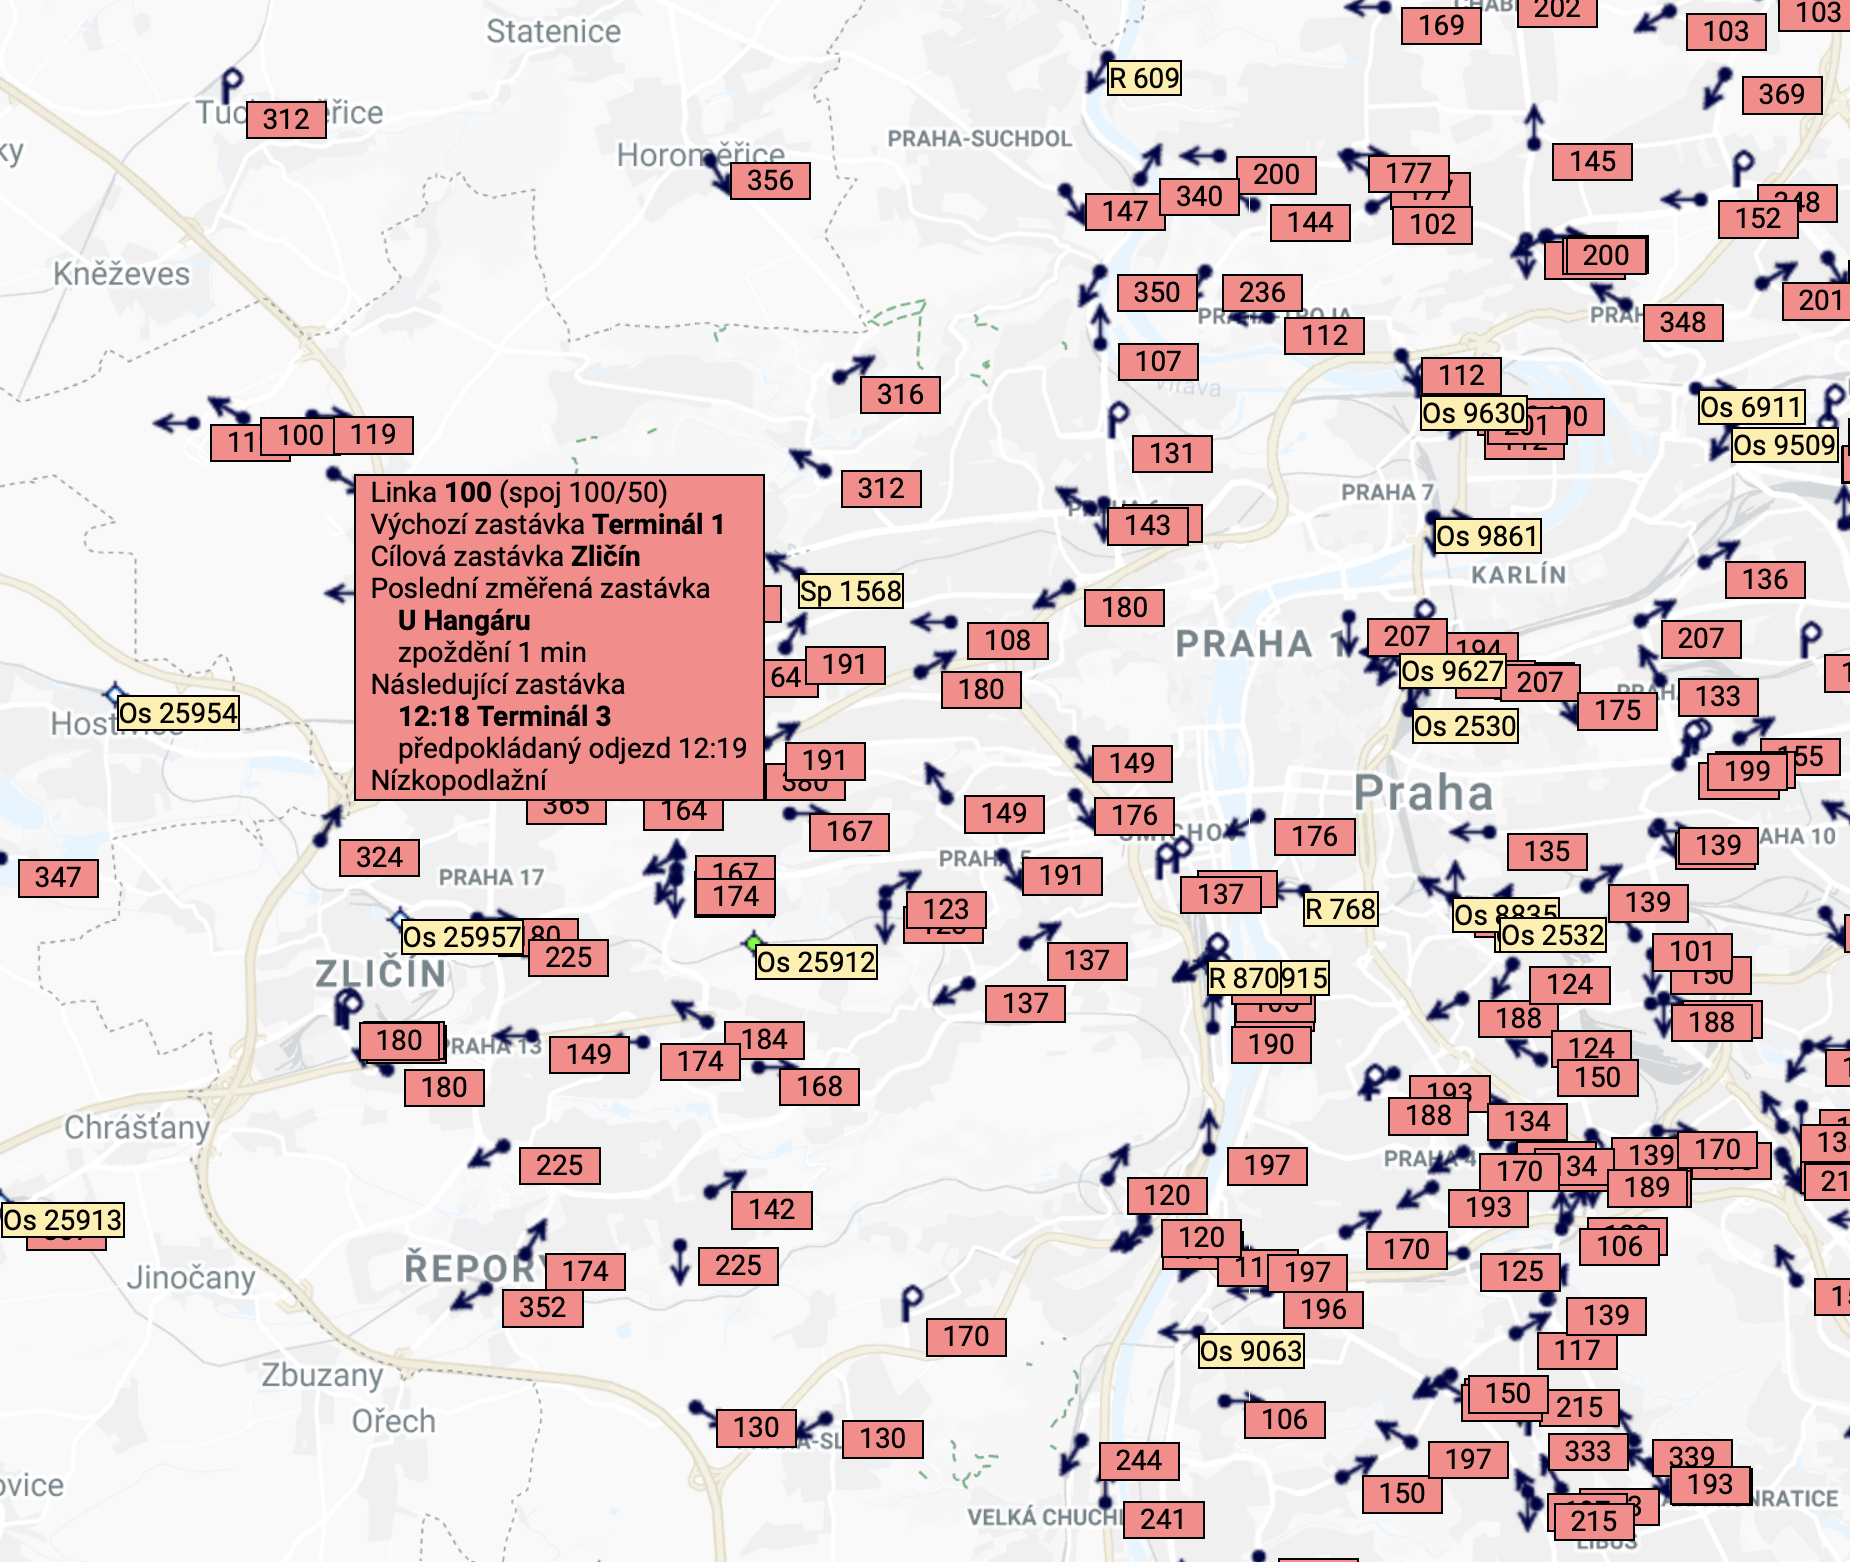
\includegraphics[width=\linewidth]{../img/tram-bus_mapa.png}
  \caption{Mapa z www.tram-bus.cz.}
  \label{fig:tram-bus_result}
\end{figure}

\subsubsection{\gls{idsjmk}}

Mimo Prahu je velice pěkně udělaná aplikace pro zobrazení vozidel \gls{idsjmk} (Integrovaný dopravní systém Jihomoravského kraje). Ten ihned po načtení stránky zobrazuje všechny dobravní prostředky, tedy tramvaje, autobusy a vlaky vše s čísly linek. Dále pak umožňuje po kliknutí na vybraný spoj zobrazit více informací včetně jízdního řádu.

\bigbreak

Tato aplikace je po vizuální i funkční stránce dobrou inspirací pro tvorbu aplikace v této práci.

\begin{figure}
  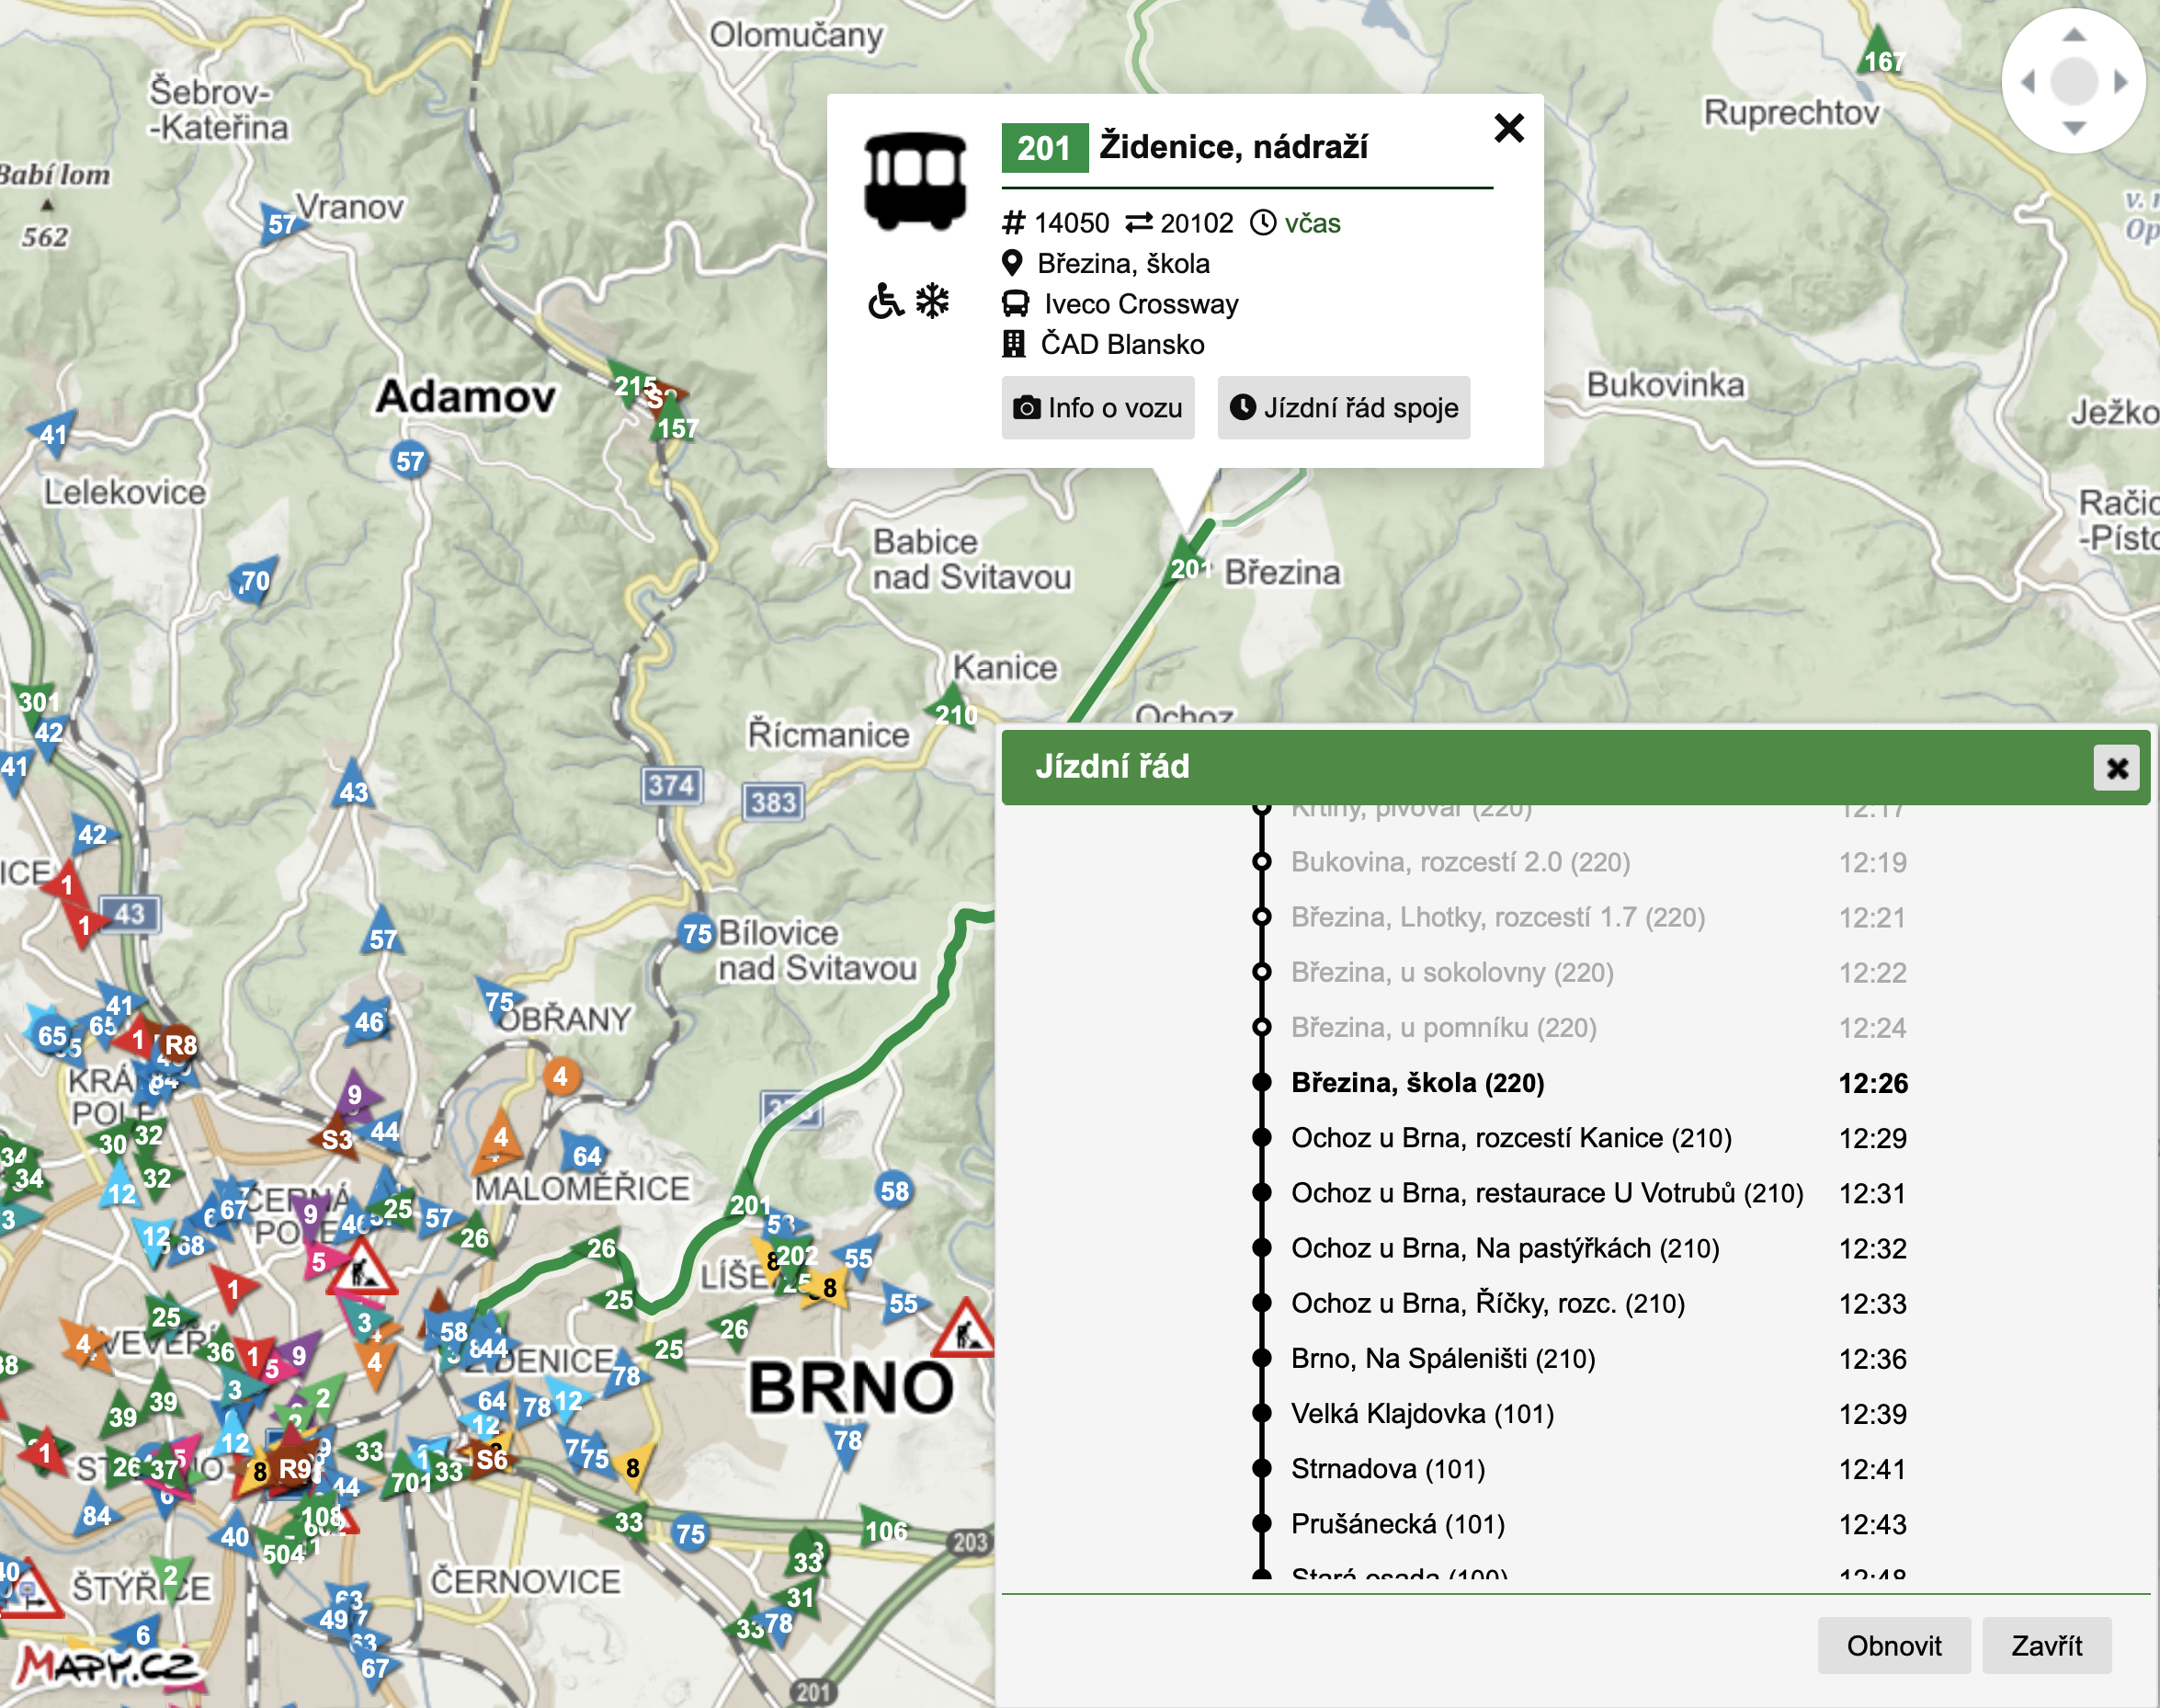
\includegraphics[width=\linewidth]{../img/idsjmk_mapa.png}
  \caption{Mapa z mapa.idsjmk.cz.}
  \label{fig:idsjmk_result}
\end{figure}
